This section provides a detailed illustration about the proposed solution of the problem discussed in the problem definition. The proposed solution consists of a redesigned architecture of the group signature scheme according to the requirements discussed in the description of the problem. The solution also incorporates remodeling various algorithm and protocols of the group signature scheme to satisfy the requirements for an efficient system. The problem definition describes a group signature where the privacy of the group members is more secure than other signature schemes. In the literature survey, we have seen the shortcomings of various group signature schemes which include the privacy concerns about the role of the sole authority of the Group Manager. The Group Manager possesses an enormous power in almost all group signature schemes. The misuse of the capability of the Group Manager can lead to exposure of the privacy of the users with the Group Manager who can make this information public.

The ability of the Group Manager to provide private key to a new member also enables him to store that key and use it for framing any user.  That's why the group signature scheme is required to implement a mechanism for join procedure in such a way that the Group Manager should not get the knowledge of the private key of the new member. The application of the Diffie Hellman key exchange can be derived in the configuration of a protocol which uses the discrete logarithm problem to interchange information between the potential member and the Group Manager. In this protocol, the Group Manager does not get the actual information instead he gets the number in such a way that to extract the information the Group Manager required to solve the discrete logarithm problem. From the Diffie Hellman assumption, we can believe that solving such problem is not possible for the Group Manager and hence the joining of the member can be performed more securely. 

Also dividing Group Managers complete task into multiple authorities and maintaining efficient correlations between them can provide enough trust to the users of the group signature scheme so they can assume that no single authority has sufficient power to produce an effect on the privacy of the signers. The following section describes the implemented solution for limiting the power of Group Manager by distributing the task into multiple authorities.

\section{Distribution of Authorities}

\index{Distribution of authorities}The power given to the Group Manager not only allows him to generate and view the private keys of the members but also provide him the ability to trace a signature to its original signer. Also in some schemes which support revocation of members, the Group Manager is solely responsible for the task of revocation. This huge amount of power may concern users of the group signature scheme about their privacy therefore we need to limit the power of Group Manager. This limitation can be accomplished by distributing the tasks of the Group Manager into three different authorities. 

\subsection{Group Manager}
\index{Distribution of authorities!Group Manager}The Group Manager as one of the authorities can add a new member to the group by providing him a private key for generating his individual signature. The private key of the group is distributed in such a way that the only section required to generate the private key of the members should be in possession of the Group Manager and this private key cannot perform other tasks like opening a signature. The private key of the potential member can be provided using the techniques of discrete logarithm discussed in the earlier section so that the Group Manager does not get the knowledge of actual key which limits the power of Group Manager and restricts him from framing attack or coalition attack. Some other duties of the Group Manager may include supervision of the activities of the group, handling disputes and transferring opening requests to the Open Manager and revocation requests to Revocation Manager. The Group Manager can also act as the administrator of the network framework of the group.

\subsection{Opening Manager}
\index{Distribution of authorities!Opening Manager}The task of the opening of the signature is assigned to a separate authority known as the Opening Manager. The Opening Manager must be the only authority having the ability to associate a group signature to its original signer. The Opening Manager should only have a particular section of the private key of the group by which he can open any signature but can not generate private keys for any new members like Group Manager. The opening of the signature provides enough identification of the user so that the Opening Manager is able to correlate the signature in question with a unique member. The revocation of a particular signer also required this secret identification of the member to revoke him. Therefore the Open Manager can send the identification of the signer of an opened signature to the Revocation Manager, but the Open Manager himself should not be able to revoke any member. In short, the Open Manager can not add or revoke any new member but only can open a signature and send the identification of the signer to Revocation Manager for cancelling the membership of a signer or solve any dispute regarding the identity of the signer. 

\subsection{Revocation Manager}
\index{Distribution of authorities!Revocation Manager}The Revocation Manager requires being in possession of only the power of revocation of the group members. The task of the Revocation Manager is to revoke a user because of various reasons according to the policy of the group. The Revocation Manager is the authority responsible for doing the judgment of actions of a signer and deciding whether a signer member should be revoked or not and if the decision is to cancel the membership of that member then the Revocation Manager revoke him.  The identification of the members is required for their revocation which is obtained from the Opening Manager. Therefore the distribution of the authorities is done in such a way that Opening Manager can only open a signature and get unique identification of its signer but cannot revoke him, and the Revocation Manager can revoke the signer but required his identification from the Opening Manager. Therefore an important action like revocation of a member need an agreement among at least two authorities and therefore can be considered more trustworthy than a monarch authority responsible for it. 

\section{Definition of Proposed Scheme}\label{pro:definition}
\index{Group Signature (Definition)}To design the architecture of a group signatures scheme, first, we need to define the group signature scheme formally. The formal definition provides mathematical and logical requirements along with the structure of algorithms of a group signature scheme. From the definition of the proposed group signature scheme, it is possible to implement the custom modified algorithms with proper understanding. The formal definition of group signatures scheme is given below. Note that the definition of the scheme is derived from the definitions provided in section \ref{ClassificationGroupSignatures}.

\begin{definition}[Group Signature]\label{def:group signature}
A group signature is a modified adaptation of digital signatures which produces a numeric string as a signature for a signer by taking an input of a message $M$ and the private key of the signer $(msk)$. The group signature scheme must consist of following six operations.

\begin{enumerate}
\item \textbf{SetUp}: A randomized probabilistic polynomial time algorithm which produces following output when provided with security parameter $\ell$ as input.
	\begin{itemize}
	\item The public key of the group $(gpk)$.
	\item The private key of Group Manager.
	\item The private key of Opening Manager.
	\item List of group members (initially empty).
	\item List of revoked members (initially empty).
	\end{itemize}

\item \textbf{Join}: A randomized probabilistic polynomial time algorithm which establishes a protocol between Group Manager and a potential member and provides private key to the member $(msk)$ by taking the input of $(gpk)$ and the private key of Group Manager. The \texttt{Join} algorithm also add the identification of that member in the \textquotedblleft List of group members\textquotedblright.

\item \textbf{Sign}: A randomized polynomial time algorithm which generates a numeric string as a signature $S$ for a message $M$ by taking input $(M, msk)$ where $M$ is a message and $msk$ is the private key of signer member.

\item \textbf{Verify}: A deterministic polynomial time algorithm which determines the validity of the signature produced by the \texttt{Sign} algorithm by taking an input of $(gpk, M, S)$. Where $gpk$ is the public key of the group and $M$ is a message, and $S$ is the signature. The \texttt{Verify} algorithm produces a binary result \texttt{True/False}, where \texttt{True} indicates signature is valid and \texttt{False} indicates signature is invalid.

\item \textbf{Open}: A deterministic polynomial time algorithm which returns $mpk$ or group member's identification who was the original signer of signature $S$ by taking the input of private key of Open Manager And signature $S$.

\item \textbf{Revoke} A polynomial time algorithm which takes an input of members identification or $mpk$ and adds it to the \textquotedblleft List of revoked members\textquotedblright ~which changes the validity of all the signatures issued by that member to invalid when verified by the \texttt{Verify} algorithm.
\end{enumerate}
\end{definition}

The group signature scheme must be incorporating following properties.

\begin{itemize}
\item \textbf{Correctness}.  The \texttt{Sign} algorithm must always produce a signature which should always found to be valid when verified by the \texttt{Verify} algorithm.

\item \textbf{Unforgeability}. Only a group member using his private key $mpk$ should be able to produce a valid signature, and no one other than group member can generate a valid signature without knowledge of private key of any member.

\item \textbf{Anonymity}. It should not be possible to determine the identity of the actual signer of a signature $S$ by anyone except by the Opening Manager possessing a secret opening key.

\item \textbf{Unlinkability}. It must be computationally hard to decide whether given two signatures are from same signer member or not.

\item \textbf{Exculpability}. No one including Group Manager and group members should be able to generate a signature which can be traced as signature signed by another member of the group.

\item \textbf{Traceability}. The Opening Manager possessing secret opening key should always be able to link a given signature $S$ to its unique and original signer.

\item \textbf{Coalition resistance}. A coalition of group members should not be able to produce a valid signature by combining their private keys.

\item \textbf{Revocability}. Any member of the group can be removed from the group at any time, and all the past and future signature generated by that member must be identified as invalid when verified by the \texttt{Verify} algorithm.
\end{itemize}

\section{Architecture of Proposed Scheme}
\index{Architecture of Proposed Scheme}The following figure describes detailed structure of proposed group signature scheme with all the algorithms defined in the definition \ref{def:group signature}.

\begin{figure}[!h]
    \centering
    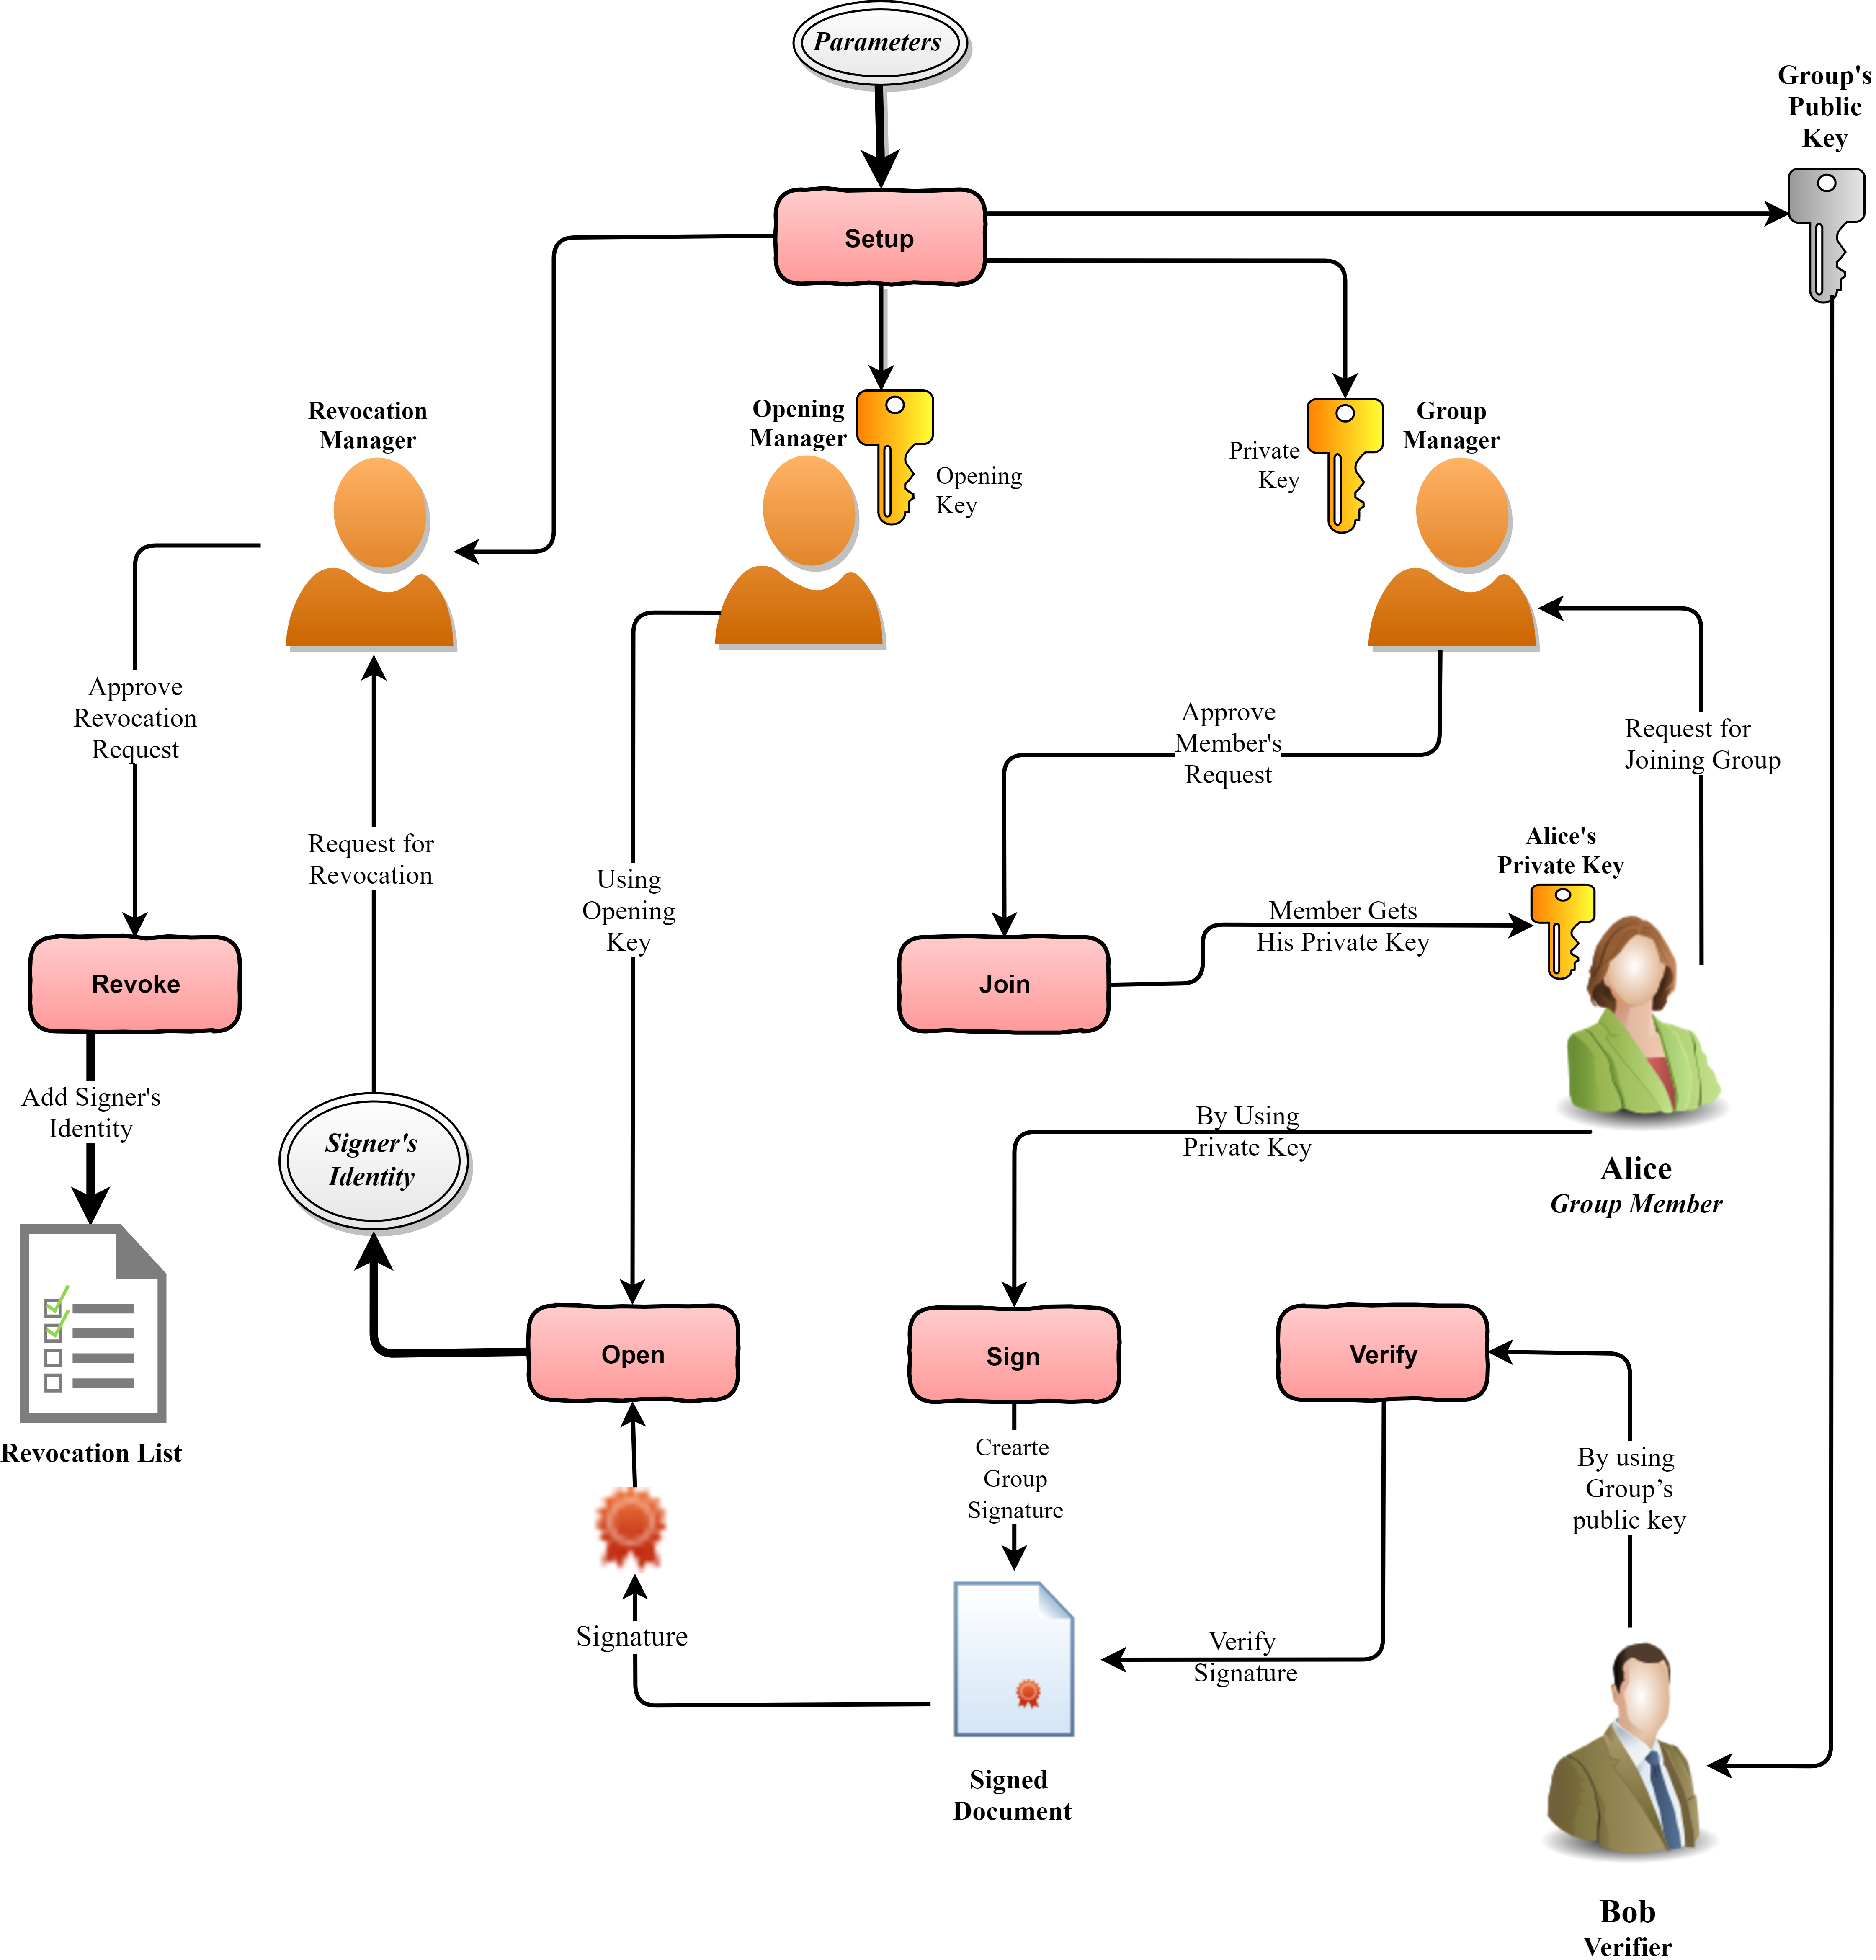
\includegraphics[width=\textwidth]{Architecture_of_group_signature}
    \caption{Architecture of Proposed Group Signatures Scheme}
    \label{fig:Architecture of Proposed Group Signatures Scheme}
\end{figure}

From the definition \ref{def:group signature}, it is simple to understand the system of proposed group signatures scheme. From the figure \ref{fig:Architecture of Proposed Group Signatures Scheme}, we can see that there are three authorities is distributed in this system viz. Group Manager, Opening Manager, and Revocation Manager. The group is started by generating and allocating private keys of the Group Manager and Opening Manager along with the public key of the group. The \texttt{SetUp} algorithm is provided input of the security parameters for generation of those keys. Once the Group Manager and Opening Manager are equipped with their private keys, the group becomes available for potential members to join. 

When a potential member Alice wants to become a member of the group, she sends a request to Group Manager for her addition in the group through the \texttt{Join} protocol. The Group Manager approves the request of the member and calculates some intermediate numbers by using his private key and transmit those numbers to Alice by using \texttt{Join} algorithm from which she can calculate her private key. Note that the private key of Alice is generated at random and the Group Manager does not have knowledge of entire key instead he has a partial knowledge of the key which can act as a unique identification of Alice. The Group Manager stores this identification of Alice in the \textquotedblleft List of group members\textquotedblright.

Once Alice gets her private key by becoming a member of the group, she can sign a message on behalf of the group. To sign a message Alice uses the \texttt{Sign} algorithm which generates a signature when provided with a message and private key of the member. Alice produces a group signature by inputting her private key and her message into the \texttt{Sign} algorithm. The signed message is then ready to be transmitted along with the signature over an insecure channel.

Bob as a non-member user of the group signature system, receives the message signed by a member of the group over an insecure channel. To verify the received message, Bob uses the \texttt{Verify} algorithm which takes an input of the message, its signature and public key of the group. The public key of the group is assumed to be available to Bob because the public key of the group is made available to all the public members either through PKI certificates or direct transmission of the certificates to potential verifiers. When Bob provides input of the received message along with its signature and the public key of the group, the \texttt{Verify} algorithm determines the validity of the signature as either valid or invalid. If the validity of the received message is found to be invalid, Bob discards the message. If the message is verified to be valid, Bob accepts the message. Note that Bob only gets information of validity of the message as is it signed by a valid member of the group or not. But Bob cannot get or determine any other information about actual signer of the message. The \texttt{Verify} algorithm also checks if the signer of the message is revoked. This procedure does not leak any information because of the use of discrete logarithm assumption in the process. If the identity of the signer is found in the \textquotedblleft List of revoked members\textquotedblright, then the \texttt{Verify} algorithm determines the validity of the message as invalid. 

In some rare cases, it is required to find out the identity of the actual signer of a message. In such cases, the message and signature are transmitted to the Opening Manager and requested to determine the identity of the original signer of that message. The Opening Manager who has a secret opening key first checks the validity of message and if the message is valid then proceed to open the message. The Opening Manager utilizes the \texttt{Open} algorithm which takes an input of signature and the private key of the Opening Manager to determine the identity of the signer. The \texttt{Open} algorithm provides the identity of the signer which is then cross referenced with \textquotedblleft List of members\textquotedblright to decide the signer of the signature. The Open Manager is the only authority holding the secret key to determine the identity of the signer. Hence no one except the Opening Manager is able to ascertain the identity of the signer of a signature. The Opening Manager sometimes needs to send the obtained identification to the Revocation Manager to revoke the membership of the signer.

Revocation Manager when received the identification of the signer, can revoke his membership. The Revocation Manager is assigned to the task of determining whether the membership of a member should be revoked or not. The Revocation Manager decides it according to the policy of the group. To revoke the membership, Revocation Manager adds the identification of the signer in the \textquotedblleft List of revoked members\textquotedblright. As we seen in the earlier paragraph, the \texttt{Verify} algorithm also checks the entries of the \textquotedblleft List of revoked members\textquotedblright for the signer while validating a message. So the messages signed by the revoked members are identified as invalid. The \textquotedblleft List of revoked member\textquotedblright is published and made available to all potential verifiers. Only the Revocation Manager have permission to modify that list and other members can only read but cannot edit the list. 

In the next section, we are going to discuss further about the algorithms of the group signature scheme in implementation point of view.

\section{Model Development}
\index{Model Development}From the definition and architecture described in the earlier section, one can see that the proposed group signature scheme is a dynamic group signature scheme with distributed authorities according to the definition \ref{def:Group Signature Scheme with Distributed Authorities} given in section \ref{sec:Group Signature Schemes with Distributed Authorities}.  To develop model according to the architecture and satisfying the definition we need to modify the algorithms and protocols of the group signature scheme. The proposed group signature scheme is based on state of the art ACJT scheme and uses the RSA assumption for its security. In the following section, we are going to describe the modified algorithms of the group signature scheme and their working.

\subsection{Security Parameters}
\index{Security Parameters}The security parameter is a variable which is used to determine the size of the input for a computational algorithm or protocol. The security parameters are used to find out the probability of breaking the security of a cryptosystem. There are several security parameters required for the scheme. Following are some security parameters which are used in various operations of our system. Also, we have used some lengths and ranges which are described below. 

Let the security parameters be $\varepsilon > 1, \ell \in \mathbb{N}, k \in \mathbb{N}$. Let $\lambda_2, \lambda_1, \gamma_2, \gamma_1$ denotes the lengths, and $\Gamma, \Lambda$ denotes integral ranges satisfying following conditions.

\tcbset{float=htb,every float=\centering, colback=white,arc=2mm, equal height group=AT,}
\begin{center}
\begin{tcolorbox}[width= 7cm, height= 7cm, valign = center]
\begin{itemize}
\item $\lambda_2 \geq 4\ell$,
\item $\lambda_1 \geq \varepsilon(\lambda_2 + k) + 2$,
\item $\gamma_2 \geq \lambda_1 + 2$, 
\item $\gamma_1 \geq \varepsilon(\gamma_2 + k)+ 2$,
\item $\Gamma =~]2^{\gamma_1-\gamma_2}, 2^{\gamma_1+\gamma_2}[$,
\item $\Lambda =~]2^{\lambda_1-\lambda_2}, 2^{\lambda_1+\lambda_2}[$.
\end{itemize}
\end{tcolorbox}
\end{center}
The parameter $\ell$ expresses the size of the modulus, and $\varepsilon$ represents tightness of zero knowledge proof. Also, let $\mathcal{H}$ be a collision resistant hash function $\mathcal{H}: \{0, 1\}^* \rightarrow \{0, 1\}^k$.

\subsection{Set Up Algorithm}
\index{Model Development!SETUP}The SetUp algorithm is executed at the very beginning of the group. The SetUp algorithm requires the parameter $\ell$ as an input for deciding the size of factors of RSA modulus $n = pq$ where $p = 2 p^\prime + 1$, $q = 2 q^\prime + 1$ and $p, p^\prime, q, q^\prime$ are all prime integers. The algorithm for SetUp operation is given below.

\begin{algorithm}
\caption{\texttt{SETUP} algorithm}
\begin{algorithmic}[1]
\vspace{10pt}
\STATE Group Manager select a special RSA modulus $n$ by selecting two random $\ell _p$ bit prime $p^\prime$ and $q^\prime$.
\STATE Generate random numbers $g, a, a_0 \in \operatorname{QR}(n)$ and of order $p^\prime q^\prime$.
\STATE Open Manager select a secret random number $x$ of size  $2\ell_p - 1$ and set it as his secret opening key 
\begin{center}
\framebox[1.1\width]{$\mathcal{S}_{om} = (x)$}
\end{center}
\STATE Open Manager get $(g,n)$ from Group Manager and calculate $y = g^x(mod~n)$ and send $y$ to Group Manager.
\STATE Group Manager sets group's public key as 
\begin{center}
\framebox[1.1\width]{$\mathcal{Y} = (n, a, a_0, y, g)$}
\end{center}
\STATE Group Manager sets group's private key as 
\begin{center}
\framebox[1.1\width]{$\mathcal{S}_{gm} = (p^\prime, q^\prime)$}
\end{center}
\vspace{10pt}
\end{algorithmic}
\end{algorithm}

From the above algorithm, we can see that at least Group Manager and Opening Manager are required for execution of SetUp algorithm. The  SetUp of algorithm generates the public key of the group as well as private keys of the Group Manager and Opening Manager. The SetUp operation is required to be executed in trusted manner. Therefore the elements $g, a, a_0$ must be generated by a cryptographically secure random number generator and factorization of $n$ should always be kept in secret. The requirement of elements $g, a, a_0$ in $QR(n)$ is for ensuring trust in the public key of the group without any need of zero knowledge proofs. The private key ${S}_{om}$ is kept secret by the Opening Manager and ${S}_{gm}$ is by Group Manager. The public key of the group is made available through common mediums like certificate signed by a trusted party.
\subsection{Join Protocol}\label{subsec:Joinalgo}
\index{Model Development!JOIN}After generating the public key of the group and private keys of the trusted authorities, the group becomes accessible for potential members to join. The Join protocol is required to be executed using secure communication channels so that any eavesdropper should not be able to get any knowledge of the private key of a member. The algorithm of the Join protocol is as follows.

\begin{algorithm}
\caption{\texttt{JOIN} algorithm}
\begin{algorithmic}[1]
\vspace{10pt}
\STATE User $U_i$ generate random exponent $\hat{x}_i \in_R ]2, 2^{\lambda_2}[$ then send $C_1 = g^{\hat{x}_i}(mod~n)$ to Group Manager. also proves his knowledge of $C_1$.
\STATE Group Manager verifies $C_1 \in \operatorname{QR}(n)$, if verified, then selects $\alpha_i$ and $\beta_i$ $\in_R ]2, 2^{\lambda_2}[$ and sends $\alpha_i$ and $\beta_i$ to user $U_i$.
\STATE User $U_i$ computes
\begin{center}
\framebox[1.1\width]{$x_i = ( \alpha_i \hat{x}_i + \beta_i (mod~2^{\lambda_2})) + 2^{\lambda_1}$}
\end{center}
and sends value of $C_2 = a^{x_i}(mod~n)$.
\STATE Group Manager checks $C_2 \in \operatorname{QR}(n)$. If it is, then selects a random prime $E_i \in_R \Gamma$ and calculate
\begin{center}
\framebox[1.1\width]{$A_i = (C_2 a_0)^{E_i^{-1}} (mod~n)$}
\end{center} 
and sends $U_i$ membership certificate $[A_i, E_i]$.
\STATE Group Manager also Stores $[A_i, E_i]$ in List of group members along with other information of the user $U_i$ like Name.
\STATE User $U_i$ verifies if 
\begin{center}
\framebox[1.1\width]{$a_0 a^{x_i} = A_i^{E_i} (mod~n)$}
\end{center} 
\vspace{10pt}
\end{algorithmic}
\end{algorithm}

From the above algorithm, we can clearly see that the use of zero knowledge protocol authenticates both the Group Manager and members. The member sends request to Group Manager for joining him into the group. Note that the $x_i$ is always hidden from Group Manager instead he only knows $a^{x_i} (~mod n)$ from which calculating $x_i$ is computationally hard. The member also validates the received certificate so no certificate can be issued without knowledge of potential member. The Group Manager also stores the certificate $[A_i, E_i]$ so that identity of user $U_i$ can be obtained later.

\subsection{Sign Procedure}\label{pro:sign}
\index{Model Development!SIGN} A member can generate a group signature for a message after becoming the member of the group by receiving his private key. The generated signature is anonymous and unlinkable to the signer. The following Sign algorithm required an input of the message for which the group signature is being generated and the private key of the member.

\begin{algorithm}
\caption{\texttt{SIGN} algorithm}
\begin{algorithmic}[1]
\vspace{10pt}
\STATE Get input of message $M \in \{0, 1\}^*$ and generate random number $w \in_R \{ 0,1 \}^{2\ell_P}$ and calculate commitments as
\begin{eqnarray*}
\left\lbrace
  \begin{aligned}
T_1 &= A_i y^w (mod~n),\\
T_2 &= g^w (mod~n),\\
T_3 &= T_2^{E_i}(mod~n).
\end{aligned}
  \right\rbrace
\end{eqnarray*}
%**
\STATE Generate random number
$r_1 \in_R \pm \{ 0,1 \}^{\varepsilon(\gamma_2 + k)}$, 
$r_2 \in_R \pm \{ 0,1 \}^{\varepsilon(\lambda_2 + k)}$, 
$r_3 \in_R \pm \{ 0,1 \}^{\varepsilon(\gamma_1 + 2\ell_p + k + 1)}$
and calculate challenges as
%**
\begin{eqnarray*}
\left\lbrace
  \begin{aligned}
d_1 &= T_1^{r_1} / a^{r_2}y^{r_3} (mod~n),\\
d_2 &= T_2^{r_1} / g^{r_3} (mod~n),\\
d_3 &= T_2^{r_1} (mod~n).
\end{aligned}
  \right\rbrace
\end{eqnarray*}
%**
\begin{center}
\framebox[1.1\width]{$C = \mathcal{H}(g|| y|| a_0 || a|| T_1|| T_2|| T_3|| d_1|| d_2|| d_3|| M)$}
\end{center}
and responses as
\begin{eqnarray*}
\left\lbrace
  \begin{aligned}
s_1 &= r_1 - C(E_i- 2^{\gamma_1}),\\
s_2 &= r_2 - C(x_i- 2^{\lambda_1}),\\
s_3 &= r_3 - C E_i w.
\end{aligned}
  \right\rbrace
\end{eqnarray*}
\hfill all in $\mathbb{Z}_n^*.$
\STATE Output generated signature as tuple: 
\begin{center}
\framebox[1.1\width]{$(C, s_1, s_2, s_3, T_1, T_2, T_3)$}
\end{center}
\vspace{10pt}
\end{algorithmic}
\end{algorithm}

The Sign algorithm generates a random number $w$ and calculates the commitments $T_1, T_2$ and $T_3$. From the above algorithm, we can see that the Sign algorithm uses an adaptation of Schnorr identification protocol and signature of knowledge from sections \ref{subsection:Schnorr Identification Protocol} and \ref{subsection:Signature of Knowledge} to produce publicly verifiable signatures. It generates random challenges $d_1, d_2$ and $d_3$ then calculate $C$ a fixed size hash digest of length $k$ from collision resistant hash function. The responses $s_1, s_2$ and $s_3$ are calculated using the private key of members and the calculated hash digest $C$. The employed hash function not only limits the value of  $C$ to a fixed size but also act as a random oracle generating random responses. The signature generated contains the hash digest $C$, commitments $T_1, T_2, T_3$ and responses $s_1, s_2, s_3$ which can be verified by a verifier. Next algorithm shows how this group signature is verified.
\subsection{Verify Procedure}
\index{Model Development!VERIFY}A receiver receives the signed message along with the output of Sign algorithm as a signature, and the public key of the group is also available to the verifier. The description of Verify algorithm which requires the message, its signature and public key of the group is as follows.

\begin{algorithm}
\caption{\texttt{VERIFY} algorithm}
\begin{algorithmic}[1]
\STATE Calculate $C^\prime = \mathcal{H}(g\parallel y\parallel a_0 \parallel a\parallel T_1\parallel T_2\parallel T_3\parallel
\frac{(a_0^C T_1^{s_1-C2^{\gamma_1}})} {(a^{s_2-C2^{\lambda_1}}y^{s_3})}
\parallel \frac{(T_2^{s_1- C2^{\gamma_1}})}{g^{s_3}} 
\parallel (T_2^{s_1-C2^{\gamma_1}}T_3^C
\parallel M) $.
\STATE Signature is valid if and only if $C = C^\prime$ and 
$s_1 \in \{ 0, 1\}^{\varepsilon(k + \gamma_2)+1}$,
$s_2 \in \{ 0, 1\}^{\varepsilon(k + \lambda_2)+1}$,
$s_3 \in \{ 0, 1\}^{\varepsilon(k + \lambda_1+2\ell_p + 1)+1}$.
\IF {Signature is valid}
	\FORALL {$E_i$ in Revocation List}
		\IF {$T_2^{E_i} = T_3$}
			\STATE Output : Signer is Revoked, Signature is Invalid.
			\STATE Break for loop
		\ENDIF
	\ENDFOR
	\STATE Output : Signature is valid.
\ELSE
	\STATE Output : Signature is Invalid.
\ENDIF
\end{algorithmic}
\end{algorithm}

From the above algorithm, we can see that the verify algorithm checks the responses and commitments by recreating challenges $d_1, d_2, d_3$ and generating $C^\prime$ same as $C$ in Sign algorithm but using newly recreated challenges and signature with group public key elements. The comparison of $C$ and $C^\prime$ is used to determine the validity of the signature. The signature is valid if $C = C^\prime$. If the signature is valid then the Verify algorithm cross checks the $T_2^{E_i} = T_3$ for all the $E_i$ present in the revocation list. If one of the equation found to be true, then we can assume that the signer is revoked and the signature is considered to be invalid. The Verify algorithm also uses a hash function as a random oracle. Therefore, it is impossible to generate a duplicate signature. Also, the hash function can detect even the smallest changes to the message and signature elements therefore integrity of message get checked automatically while verifying the signature. 

\subsection{Open Algorithm}
\index{Model Development!OPEN}Sometimes a signature is required to be associated with its original signer. The Opening Manager having a secret key for associating a signature uses the Open algorithm given below. The Open algorithm takes an input of signature and opening key $\mathcal{S}_{om}(x)$.

\begin{algorithm}
\caption{\texttt{OPEN} algorithm}
\begin{algorithmic}[1]
\vspace{10pt}
\STATE Verify the validity of signature by VERIFY algorithm.
\STATE Calculate $A_i$ (The identity of $U_i$) as
\begin{center}
\framebox[1.1\width]{$A_i = T_1/T_2^x$}
\end{center}
\STATE Prove $\log_gy = \log_{T_2}(T_1 / A_i ~mod~n)$.
\vspace{10pt}
\end{algorithmic}
\end{algorithm}

The Open algorithm first verifies the validity of the signature. The Verify algorithm confirms correct form of $T_1, T_2$ and authenticates that the signature has only one unique signer for a valid signature. The Open Manager calculates the $A_i$ of signer $U_i$ as his identity and cross check with List of group members to extract information of the user. The Opening Manager also proves that the extracted $A_i$ is correct by providing a zero knowledge proof. Once a signature is open, it does not mean that the signer cannot produce anonymous signature anymore. The Open algorithm only associates one signature at a time, and the extracted $A_i$ is kept secret by the Open Manager to preserve unlinkability to the other signature of the same signer.

\subsection{Revoke Method}\label{pro:revoke}
\index{Model Development!REVOKE}In a real world scenario, the cancellation of group member from the group is necessary. The revocation process not only removes the member from the group but also invalidates all the signatures issued by him. When Opening Manager associates a signer to a signed message, he can also send a request to Revocation Manager to revoke that member along with $[A_i, E_i]$ of the member.

When Revocation Manager decides to cancel a group member, he publishes the $A_i$ and $E_i$ of revoked user $U_i$ in the List of Revoked members. The Verify algorithm also cross check this revocation list for detecting signatures issued by revoked members. The Verify algorithm verifies that if signer of the message is revoked or not, by cross checking for all $E_i$ in Revocation List satisfying
\begin{center}
\framebox[1.1\width]{$T_2^{E_i}=^? T_3(mod~n)$}
\end{center}

If the equation satisfies for a value of $E_i$, then the Verify algorithm outputs that the signer of the message is revoked and signature is invalid. A predefined threshold is defined for the List of revoked members for optimized length. If and when List of revoked members crosses this threshold, the Group Manager reset the group by generating large random number $r$, such that $GCD(r, p^\prime q^\prime) = 1$ and calculate $a^\prime = a^r$, $a_0^\prime = a_0^r$, therefore for a user $i$
\begin{center}
\framebox[1.1\width]{$A_i^\prime = A_i^r = (a^{\prime x_i} a_0^\prime)^{1/E_i}(mod~n)$}
\end{center}

The Group Manager then replaces the group public key elements $a$ to $a^\prime$ and $a_0$ to $a_0^\prime$ redistributes new certificates $[A^\prime_i, E_i]$ to all  non-revoked members of the group.

\section{Implementation}
\index{Implementation}
The implementation of the proposed group signature scheme is made as web service for posting news anonymously as messages. The web service uses the backend of SQLite database and Python programming language. As the group signature scheme requires many big-integer calculations, especially exponential and modular operations, the choice of selecting Python programming language for backend development appears to be superior to other languages. For the front end of the development, the HTML5 and Bootstrap 3 CSS frameworks were used. The Bootstrap 3 provides some outstanding graphic elements and effects. Therefore, it found efficient to design more beautiful and attractive graphic interface.

The structure of implemented group signature scheme is group of authorized journalist and reporters found at the Setup operation. For setup of the group, the Group Manager and Opening Manager choose their private keys and the public keys of the group is generated as a result of setup operation. The group members as a trusted reporters can publish news anonymously, but a verifier can verify these messages as posted by the authorised group member. If the message is shared on social media, the receivers can also verify the received message. As no one can identify the original signer of any message, the identity, as well as the privacy of the signer, remain secure.

\subsection{Registration and Login}
To join the group, a user first needs to register as a new potential member. The following figures shows the registration and login form in the web service.
\begin{figure}[!h]
    \centering
    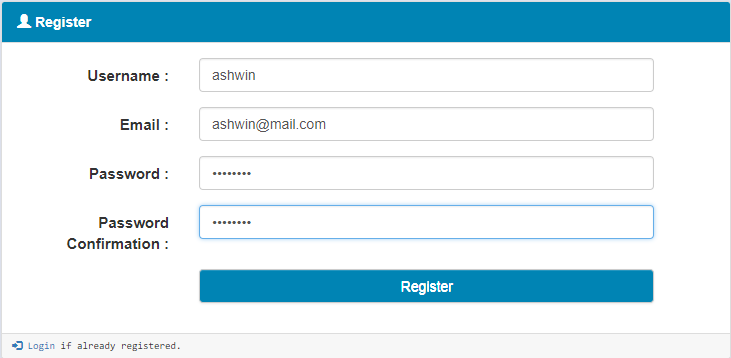
\includegraphics[width=\textwidth]{register}
    \caption{Registration Form}
    \label{fig:Registration Form}
\end{figure}

\begin{figure}[!h]
    \centering
    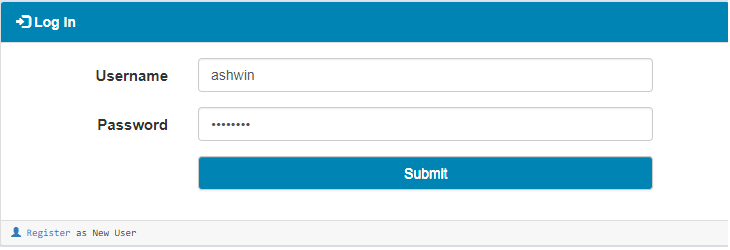
\includegraphics[width=\textwidth]{login}
    \caption{Login Form}
    \label{fig:Login Form}
\end{figure}
The registration is done by getting essential information from the user like name, email id, and password. This information is stored in the database for later reference. At the time of login, the user needs to enter his credentials like username and password for creating a login session. The username and password are compared for authentication of the user. A modern secure method of salted hashing is used to store and compare passwords in the implementation to protect password from intruders and eavesdroppers. This approach is briefly discussed in the following section.

\subsubsection{Salted Hash Passwords}
Storing passwords directly into the database is no longer remain secure as a single breach to the unsecured database by an intruder, or a hacker can lead to the breakdown of the whole implementation as passwords of all the users are known to the hackers. Encrypting the database is also not secure as it can be decrypted by various techniques simplest of it is just stealing it from the person who knows it. Also, persons having access to the database can masquerade as a different user and system do not remain secure. Simple hashing of the passwords is also not secure because of the availability of rainbow tables which contains hashes of common passwords and strings. Therefore, the concept of salted hashing is found to be most secure.

In this technique, the password of the user is first combined with some random strings called as salt. The hash of this combined string along with the salt is stored in the database. Note that the use of an HMAC for hashing is considered more secure as it requires a secret key for hashing. For authenticating a user, the password provided by him is joined with the salt, and its hash is calculated. This calculated hash it now compared with stored hash and if both the strings are equal then the password given by the user is considered as correct. This technique is resistant to brute force attack, and rainbow tables as random salt make it impossible to precompute all the possible hashes. Also by accessing the database, no one can get the passwords hence login system remains secure.

\subsubsection{Joining the Group}
Once the user gets logged in, he can formally join the group by obtaining his private key. To join the group the user clicks on the join link provided on the navigation bar. This initiates the join protocol between the user and Group Manager resulting the member getting his private key. The join operation in the implemented system is completely automatic, and only a single click is required by the user for joining the group. Once the user becomes member of the group, he can post his message in the forum by signing them.
\begin{figure}[!h]
    \centering
    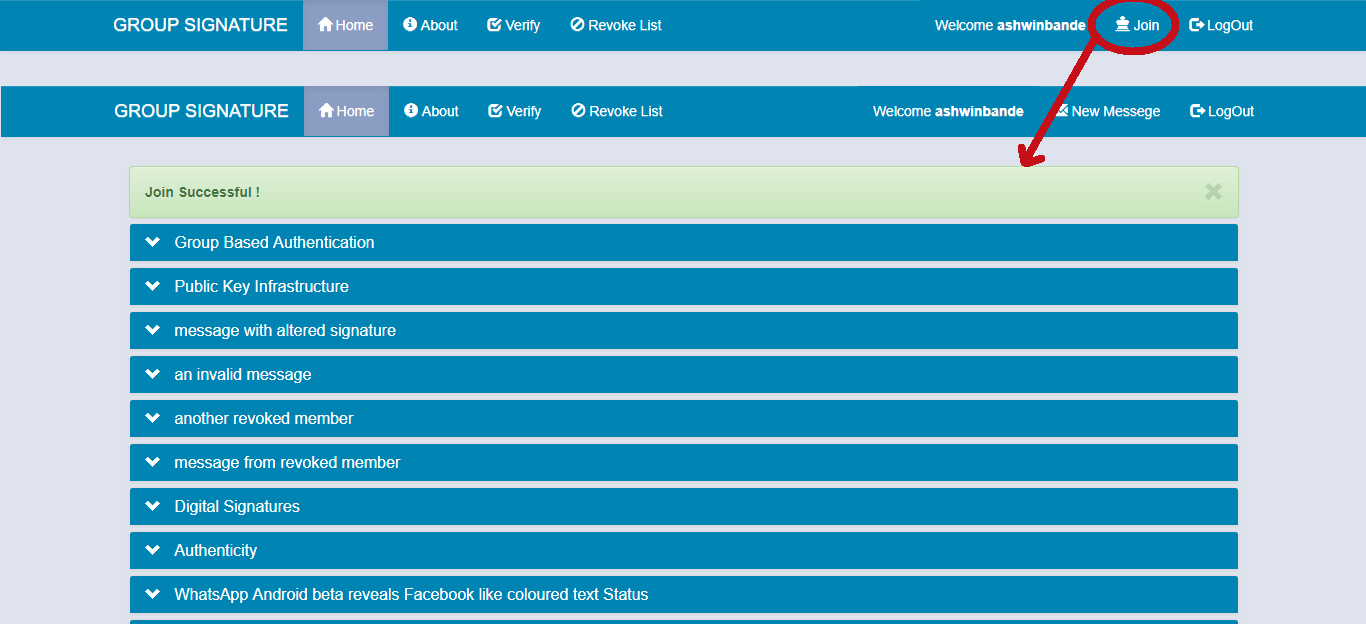
\includegraphics[width=\textwidth]{join_algorithm}
    \caption{Joining Procedure for a New Member}
    \label{fig:Joining Procedure}
\end{figure}

\subsection{Sign and Post}
To publish a message, the member first clicks on the new message and then provide the title and content of the message and click on the sign and post button. This action executes the Sign algorithm where the message and private key of the member are inputted, and the group signature for the message is calculated. The generated group signature along with the message is now published on the homepage of the website. This message can also be shared through various sharing medium like social media or through JSON\nomenclature{JSON}{JavaScript Object Notation} like data interchange format without any need for encryption. The verification of these signed messages is explained in the next section.
\begin{figure}[!h]
    \centering
    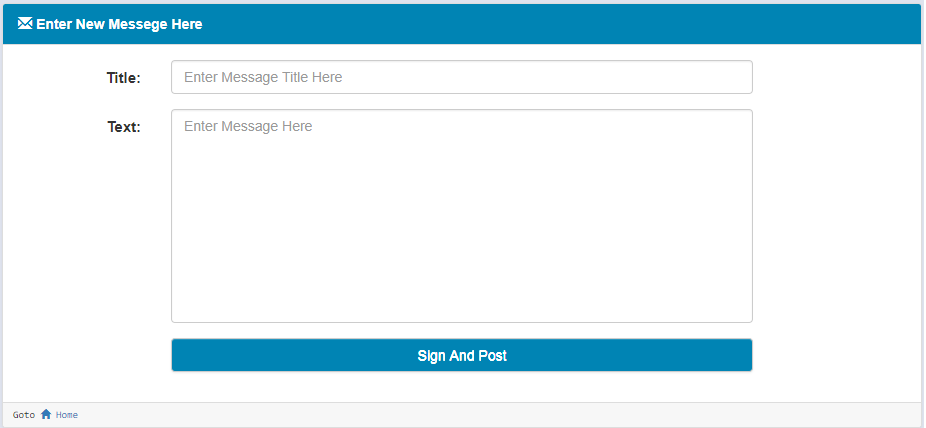
\includegraphics[width=\textwidth]{sign_and_post}
    \caption{Signing and Posting a New Message}
    \label{fig:Signing and Posting a New Message}
\end{figure}

\subsection{Verification}
\begin{figure}[!h]
    \centering
    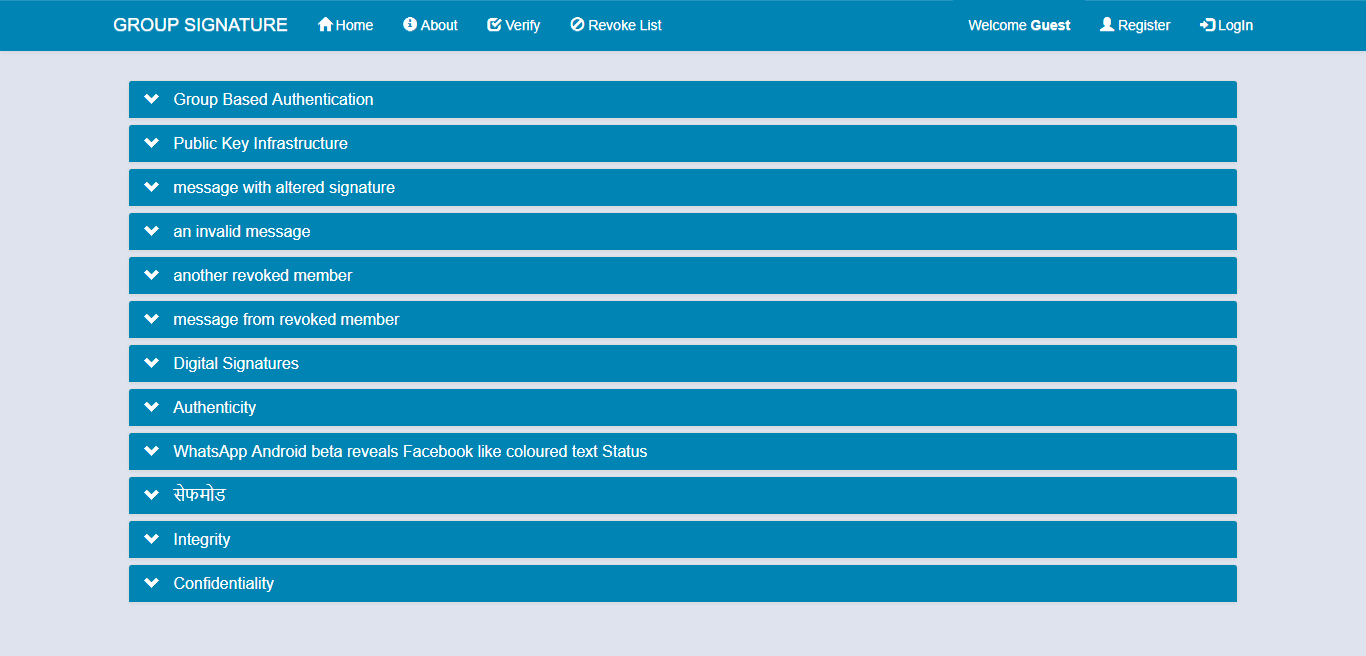
\includegraphics[width=\textwidth]{Homepage}
    \caption{Homepage of the Web Site}
    \label{fig:Homepage of the Web Site}
\end{figure}
Any verifier who wishes to verify a posted message can check it directly on the homepage. Each message contains a verify button that executes the Verify algorithm which takes an input of messages and its signature. The verifier only gets knowledge of the validity of the message as valid or invalid, but no other information is revealed during this procedure.
\begin{figure}[!h]
    \centering
    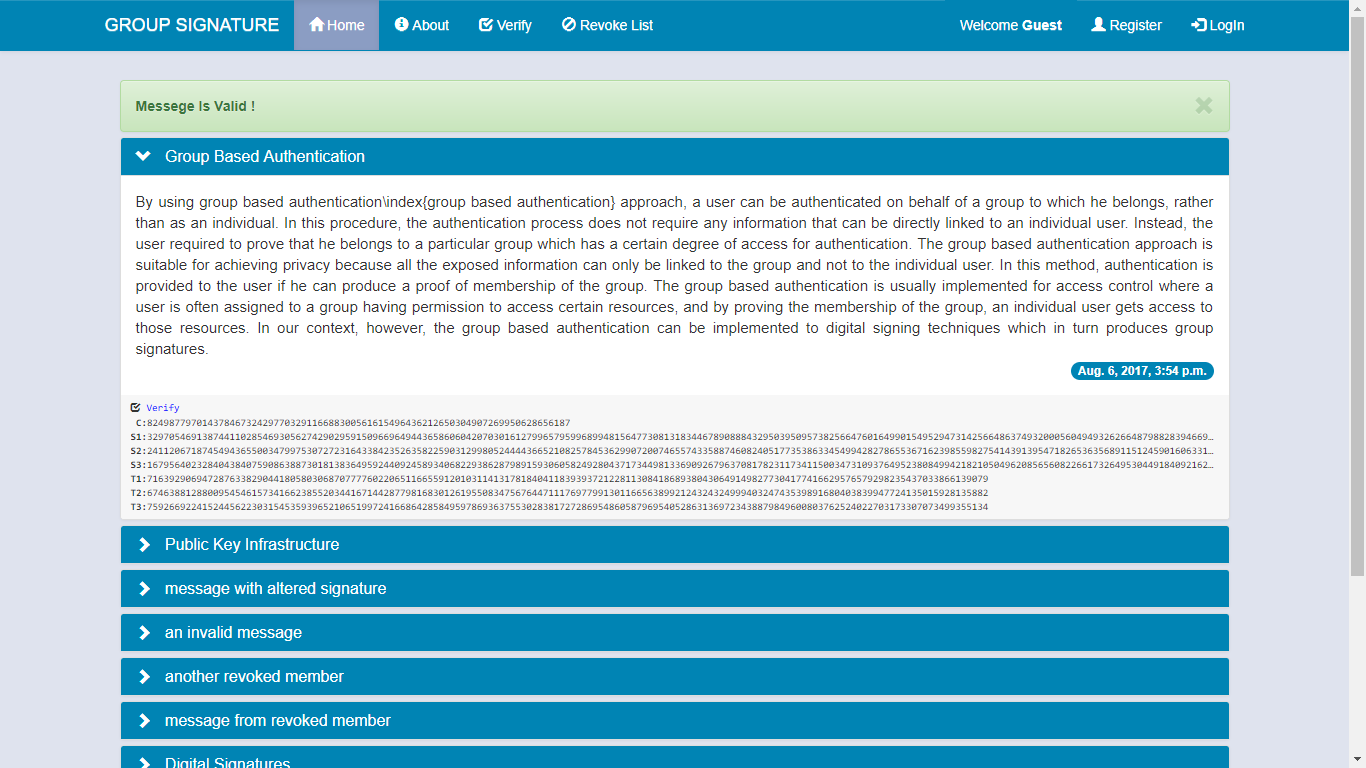
\includegraphics[width=\textwidth]{verified_message}
    \caption{Verification of a Message}
    \label{fig:Verification of a Message}
\end{figure}


\subsubsection{Revocation List}
List of revoked members is published on the web service. This list is publicly accessible and contains identities of revoked members. The Verify algorithm also cross check the signatures with this list to decide whether the revoked member signs a given signature or not. The revocation list is only accessible to the public as read only. The Revocation Manager is the only authority having the write access to the revocation list.
\begin{figure}[!h]
    \centering
    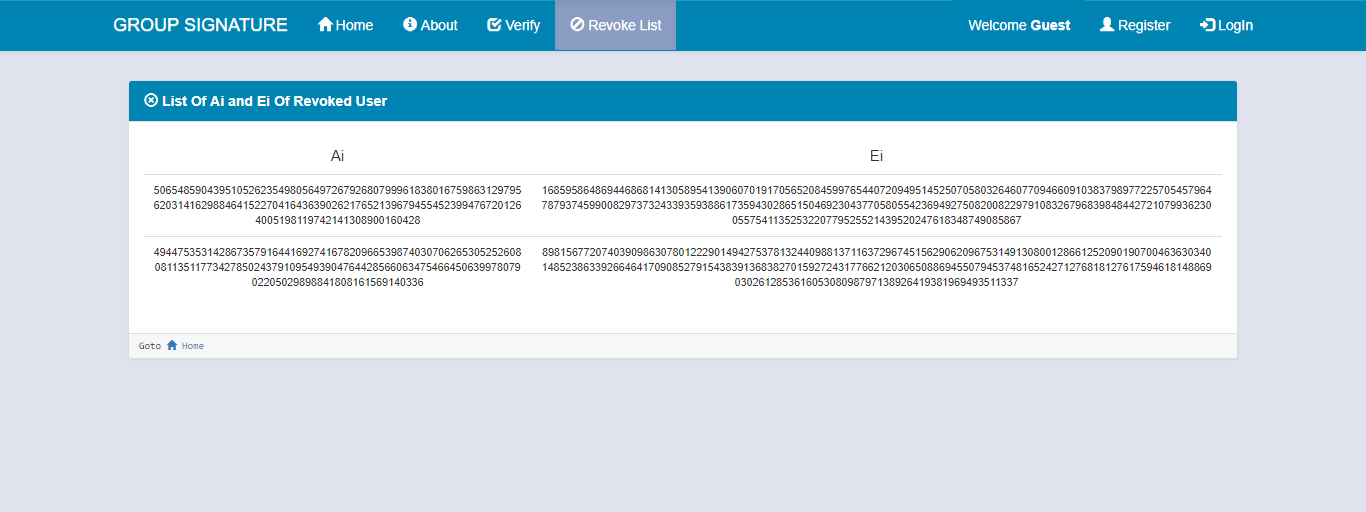
\includegraphics[width=\textwidth]{revocation_list}
    \caption{List of Revoked Members}
    \label{fig:List of Revoked Members}
\end{figure}

\subsection{Opening a Signature}
\begin{figure}[!h]
    \centering
    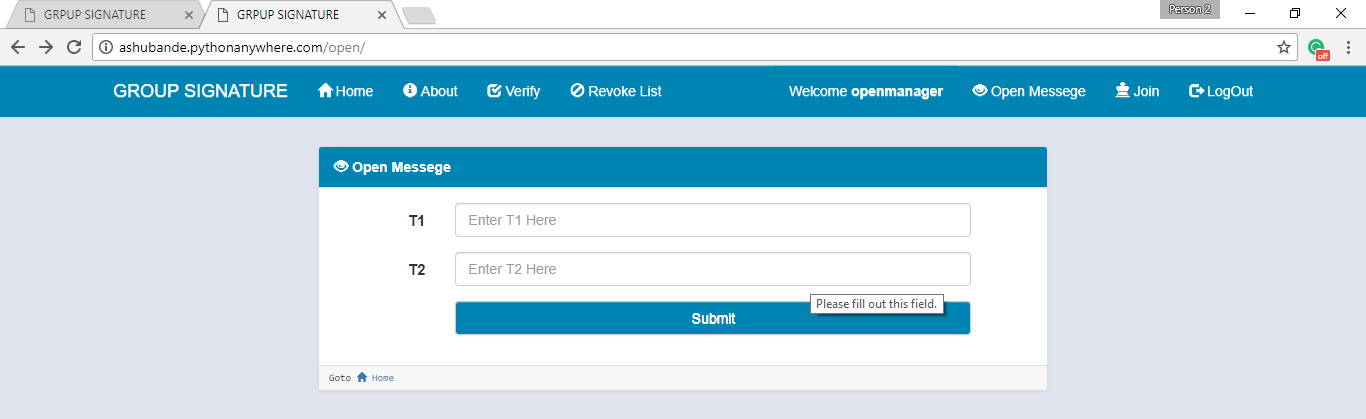
\includegraphics[width=\textwidth]{Opened_form}
    \caption{Form for Opening a Signature}
    \label{fig:Form For Opening a Signature}
\end{figure}
Sometimes the signer of a signature is needed to be identified. The Opening Manager having a specific opening key can associate a particular signature to its unique signer. The Opening Manager is provided with an exclusive option to execute the Open algorithm,  which displays a form. The form takes an input of elements $T_1, T_2$ of the signature and displays computed identity of its unique signer. The Opening Manager then can send a request for revocation of that member to the Revocation Manager. The request contains the calculated identity of the signer.
\begin{figure}[!h]
    \centering
    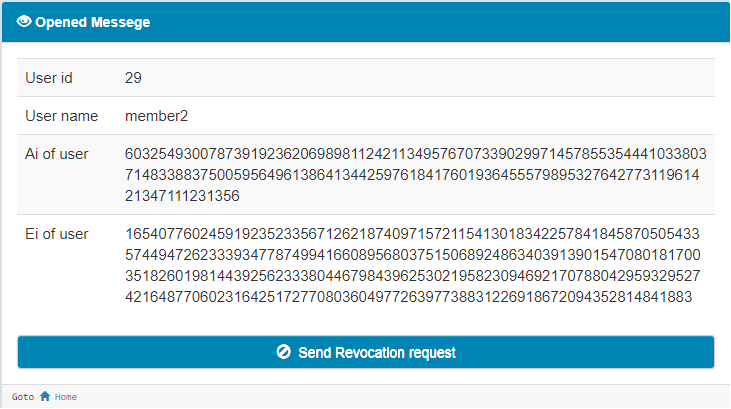
\includegraphics[width=\textwidth]{Opened_messege}
    \caption{Opened Signature of a Message}
    \label{fig:Opened Signature of a Message}
\end{figure}
\subsection{Revocation}
The Revocation Manager when receives the request of the revocation from the Opening Manager, can revoke that member. The Revocation Manager decides whether a member should be revoked or not according to the policy of the group. The Revocation Manager has two options as to accept or decline the request. If the Revocation Manager accepts the request, then the identity of the member received by the Revocation Manager is added to the list of revoked members and the Verify algorithm identifies all the message signed by that member as invalid. 
\begin{figure}[!h]
    \centering
    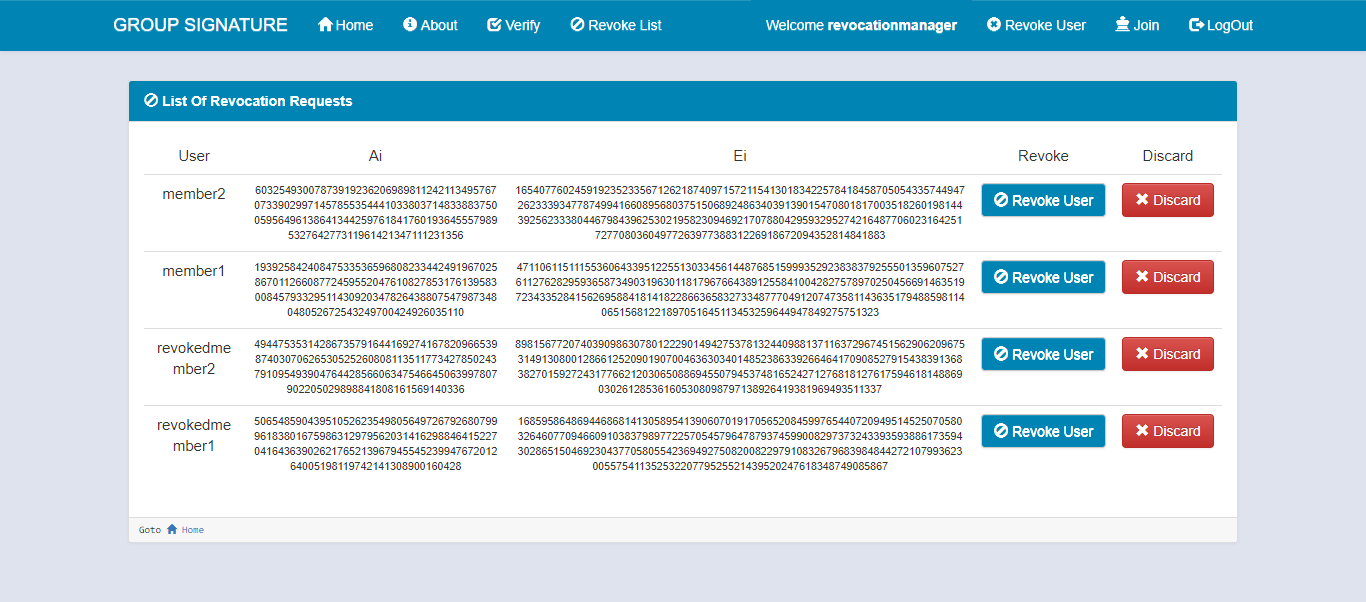
\includegraphics[width=\textwidth]{revocation_requests}
    \caption{Revocation Requests from Opening Manager}
    \label{fig:Revocation Requests from Opening Manager}
\end{figure}
